\graphicspath{{Figures/}}

\title{\fontsize{33}{45}{\huge Pattern Classification\newline{\large Lecture 07: Support Vector Machine}\newline \vspace{8pt} \Large \vspace{-1.1cm}}}

\vspace{0.5cm}
\author{\vspace{0.4cm}\\\large{\bf Kundan Kumar\\\url{https://github.com/erkundanec/PatternClassification}}
%Associate Professor\\Department of ECE}
}
% - Give the names in the same order as the appear in the paper.
% - Use the \inst{?} command only if the authors have different
%   affiliation.
%\vspace{1cm}
\institute[Indian Institute of Technology Kharagpur] % (optional, but mostly needed)
{
\vspace{1.8cm}
%\includegraphics[height=.17\textheight]{SOAlogo.png}\\
% Faculty of Engineering (ITER)\\ S`O'A Deemed to be University, Bhubaneswar, India-751030\\


 \copyright\  2020 Kundan Kumar, All Rights Reserved\\
  \vspace{-1.1cm}}
% - Use the \inst command only if there are several affiliations.
% - Keep it simple, no one is interested in your street address.
\date{}
% To remove page number from a perticular slide
{
\setbeamertemplate{logo}{}
\makeatletter
\setbeamertemplate{footline}{
        \leavevmode%
  
  % First line.
  \hbox{%
  \begin{beamercolorbox}[wd=.2\paperwidth,ht=\beamer@decolines@lineup,dp=0pt]{}%
  \end{beamercolorbox}%
  \begin{beamercolorbox}[wd=.8\paperwidth,ht=\beamer@decolines@lineup,dp=0pt]{lineup}%
  \end{beamercolorbox}%
  } %
  % Second line.
  \hbox{%
  \begin{beamercolorbox}[wd=\paperwidth,ht=\beamer@decolines@linemid,dp=0pt]{linemid}%
  \end{beamercolorbox}%
  } %
  % Third line.
  \hbox{%
  \begin{beamercolorbox}[wd=.1\paperwidth,ht=\beamer@decolines@linebottom,dp=0pt]{}%
  \end{beamercolorbox}%
  \begin{beamercolorbox}[wd=.9\paperwidth,ht=\beamer@decolines@linebottom,dp=0pt]{linebottom}%
  \end{beamercolorbox}%
  }%
        }
\makeatother
\begin{frame}
\titlepage
\end{frame}
}

\section{Introduction}
\subsection{}
\begin{frame}{}
\begin{variableblock}{\centering \Large \textbf{\vspace{4pt}\newline Linear Machine: Support Vector Machine\vspace{4pt}}}{bg=slidecolor,fg=white}{bg=slidecolor,fg=white}
\end{variableblock}
\end{frame}

\begin{frame}{Introduction}
\begin{itemize}
\item Support vector machines (SVMs) are a linear machines initially developed for two class problems, which construct a hyperplane or set of hyperplanes in a high- or infinite-dimensional space.
\item SVMs are a set of supervised learning methods used for 
\begin{itemize}
\item classification, 
\item regression and 
\item outliers detection.
\end{itemize}
\item The advantages of support vector machines are:
\begin{itemize}
\item Effective in high dimensional spaces.
\item Also, effective in cases where number of dimensions is greater than the number of samples.
\item Uses a subset of training points in the decision function (called {\color{mycolor2}support vectors}), so it is also {\color{mycolor1}memory efficient}.
\item Versatile: different SVM kernels can be specified for the decision function. Common kernels are provided, but it is also possible to specify custom kernels.
\end{itemize}
\end{itemize}
\end{frame}


\begin{frame}{Introduction}
\begin{itemize}
\item The disadvantages of support vector machines include:
\begin{itemize}
\item If the number of features is much greater than the number of samples then choosing regularization to avoiding over-fitting is crucial. 
\item SVMs do not directly provide probability estimates, these are calculated using an expensive five-fold cross-validation.
\end{itemize}
\item In addition to performing linear classification, SVMs can efficiently perform a non-linear classification using what is called {\color{mycolor1}Kernel trick}.
\item Kernel trick implicitly maps their input into high-dimensional feature space.
\end{itemize}
\end{frame}

\section{Linear Machine}
\subsection{}
\begin{frame}{Linear decision boundary}
\begin{itemize}
\item Binary classification can be viewed as the task of separating classes in feature space using decision boundary:
\begin{figure}
\includegraphics[scale=0.5]{Figures/data4.pdf}
\end{figure}
\[f({\rm x})=\text{sign}({\rm w}^T{\rm x}+b)\]
\end{itemize}
\end{frame}

\begin{frame}{What is a good Decision Boundary?}
\begin{itemize}
\item Consider a two-class, linearly
separable classification problem, many decision boundaries are possible.
\item Are all decision boundaries equally
good?
\item Which of the linear separators is optimal?
\item  The perceptron algorithm can be
used to find such a boundary.
\end{itemize}
\begin{figure}
\includegraphics[scale=0.43]{Figures/data2.pdf}
\end{figure}
\end{frame}

\begin{frame}{Linear SVM: Objective}
\begin{itemize}
\item Let us training data set, $\mathcal{D}$, a set of $n$ points.
\[\mathcal{D}=\{({\rm x}_i,y_i)~~|~~{\rm x}_i\in \Re ^d, y_i\in \{-1,1\}\}^n_{i=1}\]
${\rm x}_i~~\rightarrow$~~$d$-dimensional real vector
\item {\color{mycolor2} Objective}: find maximum-margin hyperplane 
\[{\rm w}^T{\rm x}+b=0\]
where ${\rm w}$ is the normal vector to the hyperplane and $b$ is the bias/intercept.
\begin{figure}
\includegraphics[scale=0.3]{data0}~~~
\includegraphics[scale=0.3]{data1}
\end{figure}
\end{itemize}
\end{frame}


\begin{frame}{Linear SVM: pictorial representation}
\begin{figure}
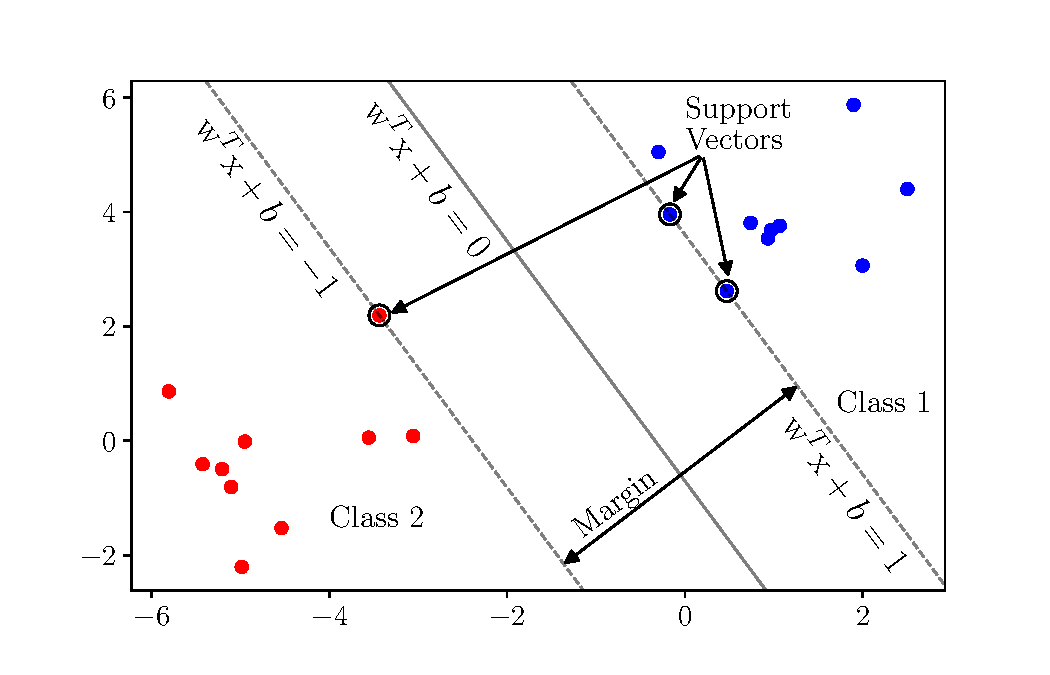
\includegraphics[scale=0.55]{Figures/data5}
\end{figure}
\end{frame}

\begin{frame}{Preliminary concepts}
\begin{itemize}
\item Let ${\rm x}_n$ be the nearest data point to the plane ${\rm w}^T{\rm x}+b=0$. 
\item How far is it?
\item Normalize ${\rm w}$ and $b$ such that:
\[|{\rm w}^T{\rm x}_n+b|=1\]
\end{itemize}
\begin{columns}
\begin{column}{6cm}
\vspace{-12pt}
\begin{itemize}
\item Now, we need to compute the distance between ${\rm x}_n$ and the plane ${\rm w}^T{\rm x}+b=0$, where $|{\rm w}^{T}{\rm x}_n+b|=1$.
\item The vector ${\rm w}$ is $\perp$ to the plane in the $\mathcal{X}$ space:
\item Take ${\rm x}_1$ and ${\rm x}_2$ on the plane
\[{\rm w}^T{\rm x}_1+b=0~~\text{and}~~{\rm w}^T{\rm x}_2+b=0\]
\end{itemize}
\end{column}
\begin{column}{4.5cm}
\begin{figure}
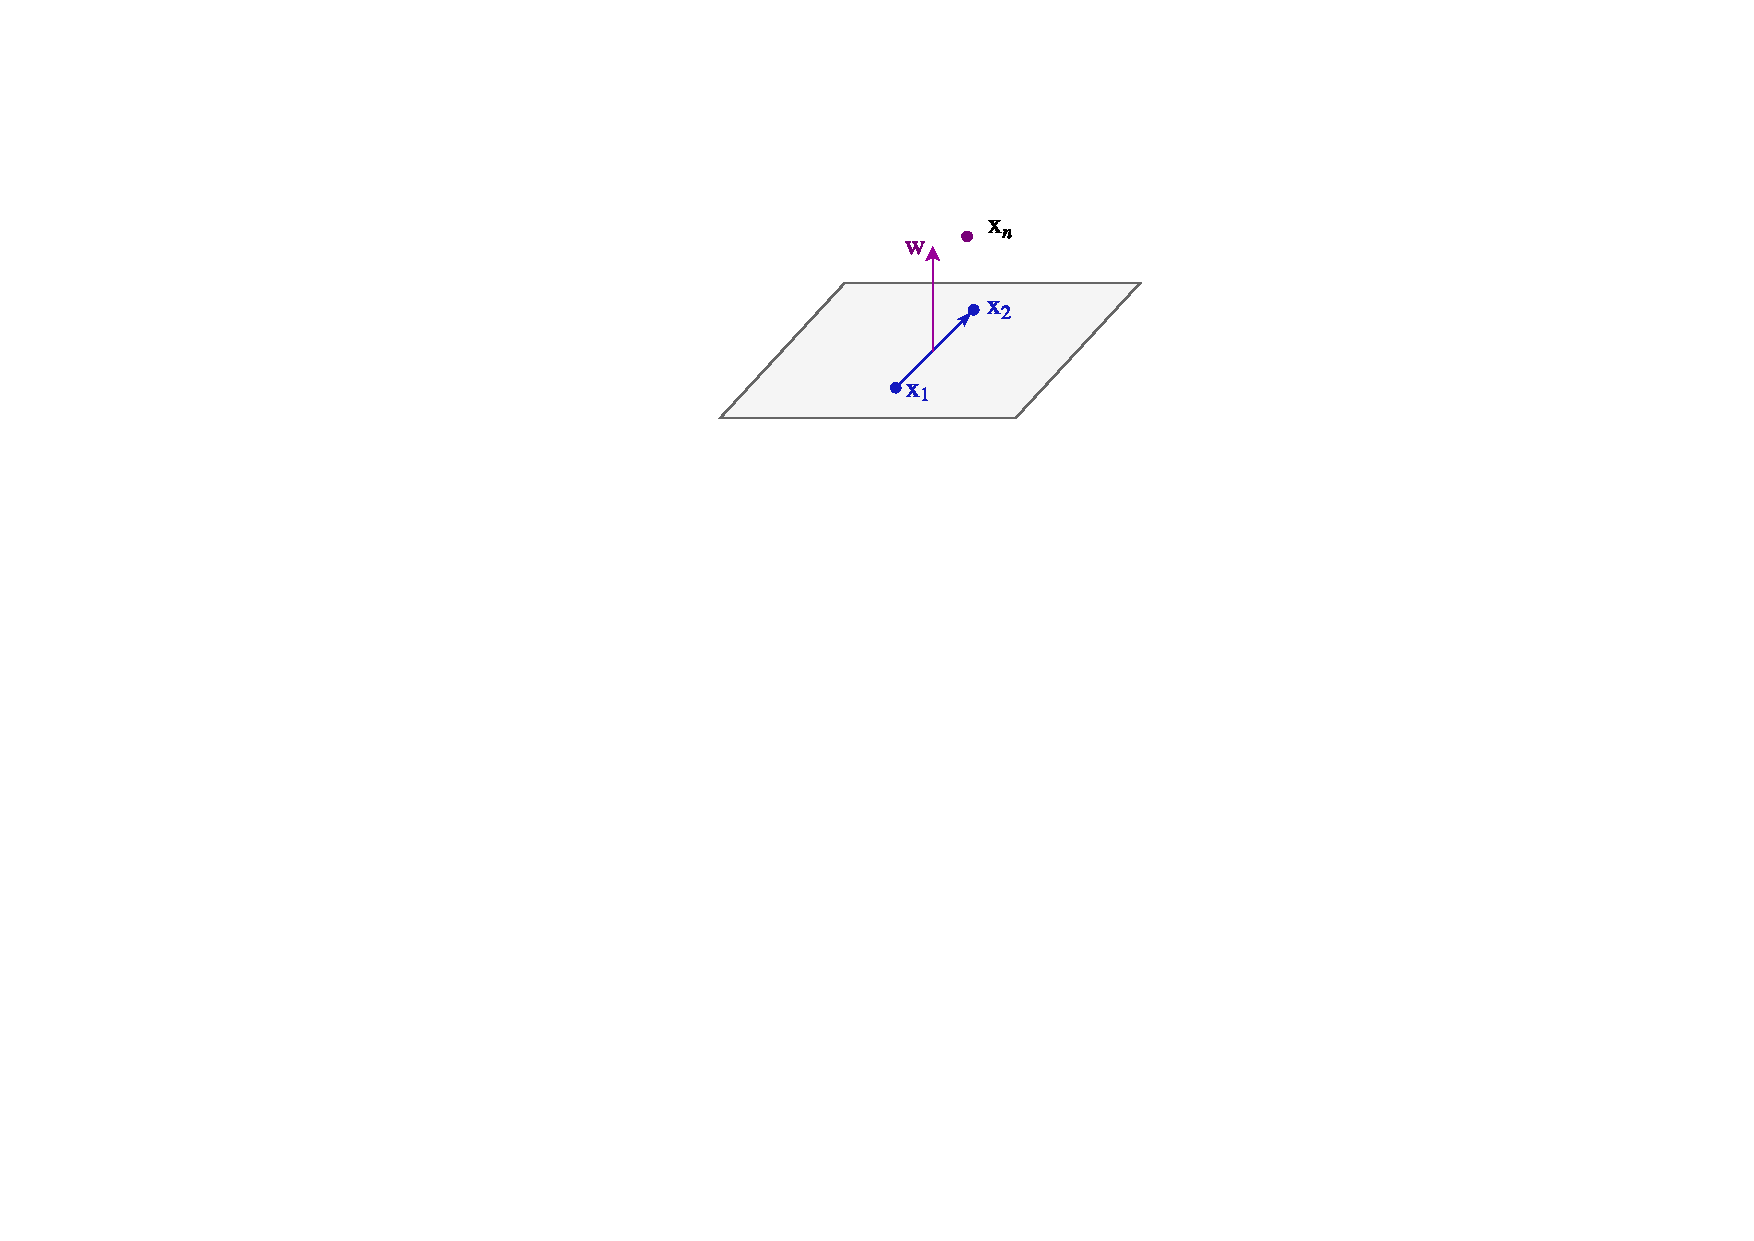
\includegraphics[scale=0.7]{SVM01}
\end{figure}
\[\Rightarrow~~ {\rm w}^T({\rm x}_1-{\rm x}_2)=0\]
\end{column}
\end{columns}
\end{frame}

\begin{frame}{Preliminary concepts}
The distance between ${\rm x}_n$ and the plane:
\begin{columns}
\begin{column}{4cm}
\begin{figure}
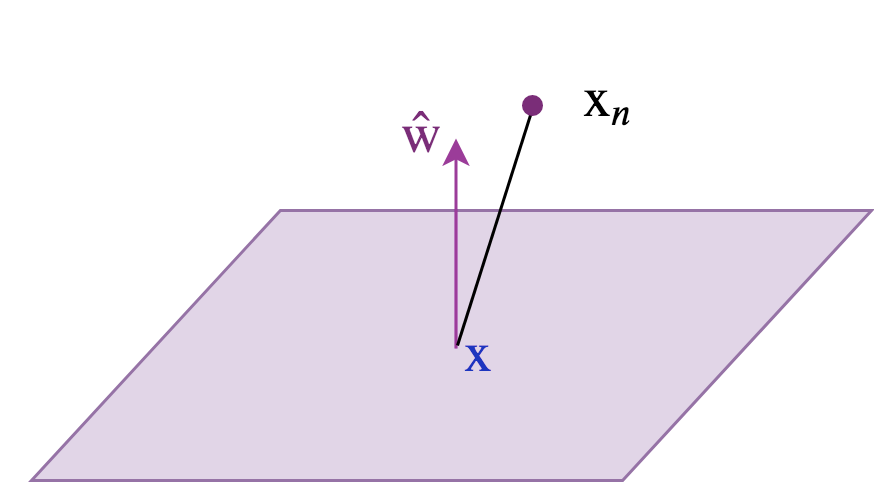
\includegraphics[scale=0.6]{Figures/SVM02.png}
\end{figure}
\end{column}
\begin{column}{6cm}
\begin{itemize}
\item Take any point ${\rm x}$ on the plane
\item Projection of ${\rm x}_n-{\rm x}$ on $\hat{\rm w}$
\[\hat{\rm w}=\frac{\rm w}{||\rm w||}\]
\[\Rightarrow ~~\text{distance}=|\hat{\rm w}^T({\rm x}_n-{\rm x})|\]
%
%${\rm w}^T{\rm x}+b=0$, where $|{\rm w}^{T}{\rm x}_n+b|=1$.
%\item The vector ${\rm w}$ is $\perp$ to the plane in the $\mathcal{X}$ space:
%\item Take ${\rm x}'$ and ${\rm x}''$ on the plane
%\[{\rm w}^T{\rm x}'+b=0~~\text{and}~~{\rm w}^T{\rm x}''+b=0\]
%\[\Rightarrow~~ {\rm w}^T({\rm x}'-{\rm x}'')=0\]
\end{itemize}

\end{column}
\end{columns}
\[\text{distance} = \frac{1}{||{\rm w}||}|{\rm w}^T{\rm x}_n-{\rm w}^T{\rm x}|= \frac{1}{||{\rm w}||}|{\rm w}^T{\rm x}_n+b-{\rm w}^T{\rm x}-b|=\frac{1}{||{\rm w}||}\]
\end{frame}


\begin{frame}{Problem formulation}
\begin{columns}
\begin{column}{6cm}
\begin{figure}
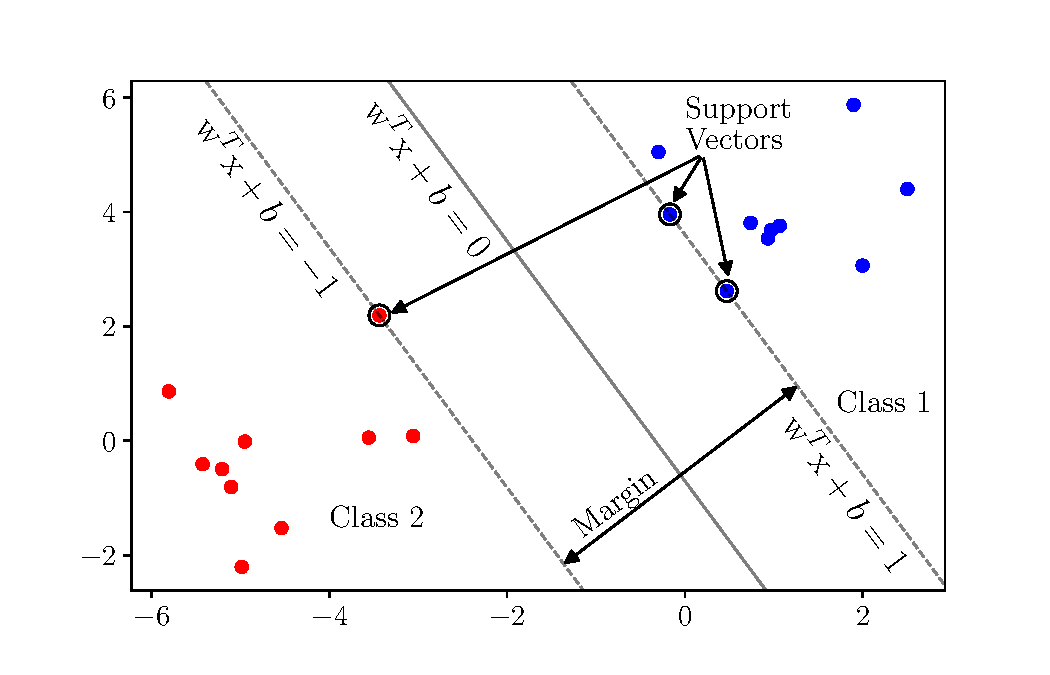
\includegraphics[scale=0.43]{Figures/data5}
\end{figure}
\end{column}
\begin{column}{5cm}

\begin{itemize}
\item Two hyperplanes
\begin{align*}
{\rm w}^T{\rm x}+b=&1\\
{\rm w}^T{\rm x}+b=&-1
\end{align*}
\item So the distance between the hyperplane is
\[\frac{b+1}{||{\rm w}||}-\frac{b-1}{||{\rm w}||}=\frac{2}{||{\rm w}||}\]
(need to be maximize)
\item Therefore, $||{\rm w}||$ need to be minimize.
\end{itemize}
\end{column}
\end{columns}
\end{frame}

\begin{frame}{Problem formulation}
\begin{itemize}
\item We need to minimize $||{\rm w}||$ to maximize the margin.
\item We also have to restrict data points from falling into the margin, so add the following constraints:
\begin{itemize}
\item ${\rm w}^T{\rm x}_i+b\geq 1$ for ${x}_i$ of the 1st class.
\item ${\rm w}^T{\rm x}_i+b\leq -1$ for ${x}_i$ of the 2nd class.
\end{itemize}
\item This can be written as
\[y_i({\rm w}^T{\rm x}_i+b)\geq 1~~~\text{for}~~~i=1,2,\ldots,n\hspace{7cm}\]
\item Combining the above two
\begin{align*}
&\mathop{\sf Minimize}\limits_{{\rm w},b}~~||{\rm w}||\hspace{6cm}\\
&\text{subject to}~~y_i( {{{\rm w}^T}{{\rm x}_i} + b} ) \geq 1~~~\text{for}~~~i=1,2,\ldots,n\hspace{6cm}
\end{align*}
\end{itemize}
\begin{tikzpicture}[remember picture,overlay]
  \node (img1) at (11,3.4) {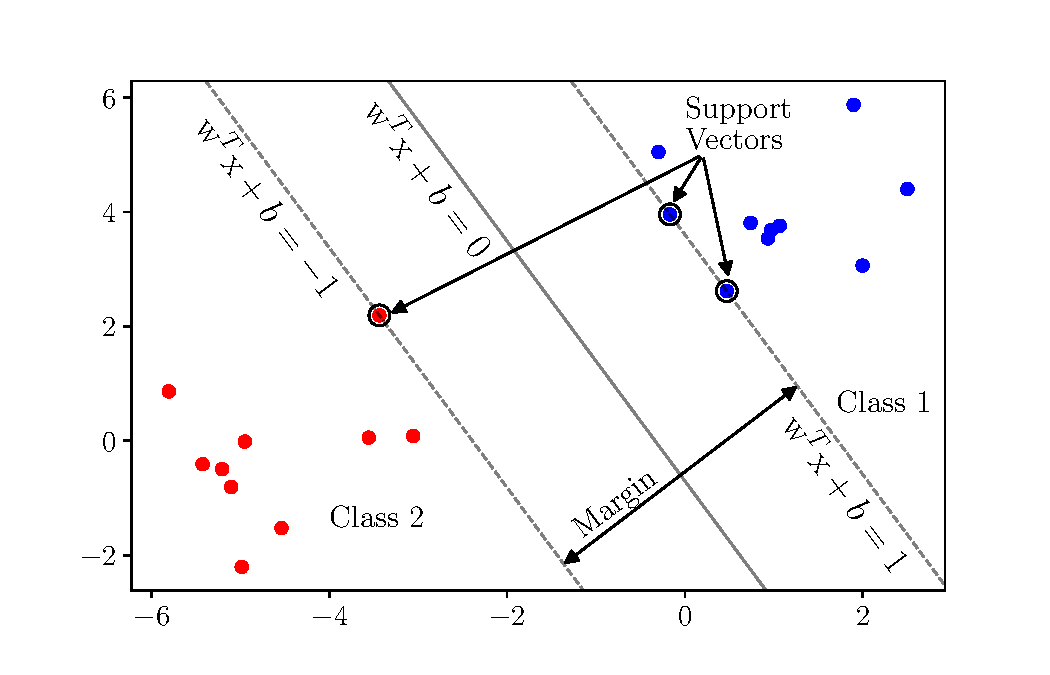
\includegraphics[height=4cm]{Figures/data5}};
\end{tikzpicture}
\end{frame}

\begin{frame}{Problem formulation}
%\begin{align*}
%&\text{Maximize}~~\frac{1}{{\left\| {\rm w} \right\|}}\\
%&\text{subject to}\mathop {\min }\limits_{n = 1,2, \ldots N} \left| {{{\rm w}^T}{{\rm x}_n} + b} \right| = 1~~~~~~~~~~~~~~~~~~~~~~~~
%\end{align*}
%Notice: $\left| {{{\rm w}^T}{{\rm x}_n} + b} \right|=y_n( {{{\rm w}^T}{{\rm x}_n} + b} )$
\begin{itemize}

\item Problem is difficult to solve because it depends on $||{\rm w}||$, the norm of ${\rm w}$, which involves a square root.
\item Substitute $||{\rm w}||$ with $\frac{1}{2}||{\rm w}||^2$ (just for mathematical convenience)
\item Then problem is formulated as

\begin{align*}
&\mathop{\sf Minimize}\limits_{{\rm w},b}~~\frac{1}{2}||{\rm w}||^2\\
&\text{subject to}~~y_i( {{{\rm w}^T}{{\rm x}_i} + b} ) \geq 1~~~~\text{for}~~~i=1,2,\ldots,n
\end{align*}
where ${\rm w}\in \Re^d$ and $b\in \Re$
\item The above problem is {\color{mycolor1}constraint optimization problem}.
\item {\color{mycolor2}Read about Lagrangian and inequality constraint KKT}\nocite{duda2012pattern}
\end{itemize}
\end{frame}


\begin{frame}{Problem solution: Lagrange formulation}
\begin{itemize}
\item There is {\color{mycolor2}no direct solution} of the formulated constraint optimization problem.
\item To obtain the dual, take positive Lagrange multiplier $\alpha_i$ multiplied by each constraint and subtract from the objective function.
\[{\sf Minimize}~~~\mathcal{L}({\rm w},b,\alpha)=\frac{1}{2}{\rm w}^T{\rm w} -\sum_{i=1}^{n} \alpha_i (y_i({\rm w}^T{\rm x}_i+b)-1)\]
w.r.t. ${\rm w}$ and $b$ and maximize w.r.t. each $\alpha_{i}\geq 0$
\item We can find the constraint as
\[\begin{gathered}
  {\nabla _{\rm w}}\mathcal{L} = {\rm w} - \sum\limits_{i = 1}^n {{\alpha _i}{y_i}{{\rm x}_i} = 0}  \hfill \\
  \frac{{\partial \mathcal{L}}}{{\partial b}} =  - \sum\limits_{i = 1}^n {{\alpha _i}{y_i} = 0}  \hfill \\ 
\end{gathered} \]
\end{itemize}
\end{frame}

%\begin{frame}{Constrained optimization}
%\begin{figure}
%\includegraphics[width=\textwidth]{SVM03}
%\end{figure}
%\end{frame}

%\begin{frame}{We saw this before}
%\begin{figure}
%\includegraphics[width=\textwidth]{SVM04}
%\end{figure}
%\end{frame}

%\begin{frame}{Lagrange formulation}
%\begin{figure}
%\includegraphics[width=\textwidth]{SVM05}
%\end{figure}
%\end{frame}

\begin{frame}{Problem solution: Lagrange formulation}
\begin{itemize}
\item We obtained
\[ {\rm w} = \sum\limits_{i = 1}^n {{\alpha _i}{y_i}{{\rm x}_i}}    ~~~~~~~ \text{and} ~~~~~~~    \sum\limits_{i = 1}^n {{\alpha _i}{y_i} = 0} \]
\item Substitute in Lagrangian optimization problem,
\[\mathcal{L}({\rm w},b,\alpha ) = \frac{1}{2}{{\rm w}^T}{\rm w} - \sum\limits_{i = 1}^n {{\alpha _i}({y_i}({{\rm w}^T}{{\rm x}_i} + b) - 1)} \]
 we get
 \[\mathcal{L}(\alpha ) = \sum_{n=1}^{n}\alpha_n -\frac{1}{2}\sum_{i=1}^{n} \sum\limits_{j= 1}^n y_iy_j\alpha_i\alpha_j {\rm x}_i^T{\rm x}_j\]
 Maximize w.r.t. to $\alpha$ subject to $\alpha_i\geq 0$ for $i=1,\ldots,n$ and $\sum_{i=1}^n\alpha_iy_i =0$
\end{itemize}
\end{frame}

\begin{frame}{The solution - quadratic programming}
\[\begin{gathered}
  \mathop {\min }\limits_{\color{blue}\alpha}  ~~~ \frac{1}{2}{{\color{blue}\alpha}  ^T}\left[ {\begin{array}{*{20}{c}}
  {{y_1}{y_1}x_1^T{x_1}}&{{y_1}{y_2}x_1^T{x_2}}&{\cdots}&{{y_1}{y_n}x_1^T{x_n}} \\ 
  {{y_2}{y_1}x_2^T{x_1}}&{{y_2}{y_2}x_2^T{x_2}}&{\cdots}&{{y_2}{y_n}x_2^T{x_n}} \\ 
  {\vdots}&{\vdots}&{\ddots}&{\vdots} \\ 
  {{y_n}{y_1}x_n^T{x_1}}&{{y_n}{y_2}x_n^T{x_2}}&{\cdots}&{{y_n}{y_n}x_n^T{x_n}} 
\end{array}} \right]{\color{blue}\alpha}  + \left( { - {1^T}} \right){\color{blue}\alpha}  \hfill \\\\
  \text{subject to   }{{\rm y}^T}{\color{blue}\alpha}   = 0\text{   and   }0 \leqslant {\color{blue}\alpha}   \leqslant \infty  \hfill \\ 
\end{gathered} \]
\end{frame}

%\begin{frame}{Substituting...}
%\begin{figure}
%\includegraphics[width=\textwidth]{SVM06}
%\end{figure}
%\end{frame}




\begin{frame}{QP hand us $\alpha$}
\begin{columns}
\begin{column}{7cm}
\begin{itemize}
\item Solution: ${\color{blue}\alpha} =\alpha_1,\ldots,\alpha_n$
\[\Rightarrow {\rm w}=\sum_{i=1}^n \alpha_i y_i {\rm x}_i\]

\item KKT condition: For $i=1,\ldots,n$
\[\alpha_i(y_i({\rm w}^T{\rm x}_i+b)-1)=0\]

\item For non-zero value of $\alpha$ ($\alpha_n>0$), ${\rm x}_n$ are support vectors.
\end{itemize}
\end{column}
\begin{column}{7cm}
\begin{figure}
\includegraphics[scale=0.45]{data1}
\end{figure}
\end{column}
\end{columns}
\end{frame}

\begin{frame}{Support vectors}
\begin{columns}
\begin{column}{7cm}
\begin{itemize}
\item Closest ${\rm x}_i$'s to the plane achieve the margin
\[\Rightarrow y_i({\rm w}^T{\rm x_i}+b)=1\]

\item We have the weight vector
\[{\rm w}=\sum_{{x_i} \text{ is SV}}\alpha_iy_i{\rm x}_i\]

\item {\color{mycolor1}Solve for $b$}: using any Support vector (SV):
\[y_i({\rm w}^T{\rm x}_i +b)=1\]
\end{itemize}
\end{column}
\begin{column}{7cm}
\begin{figure}
\includegraphics[scale=0.45]{data1}
\end{figure}
\end{column}
\end{columns}
\end{frame}

\begin{frame}{Non-separable features}
\begin{figure}
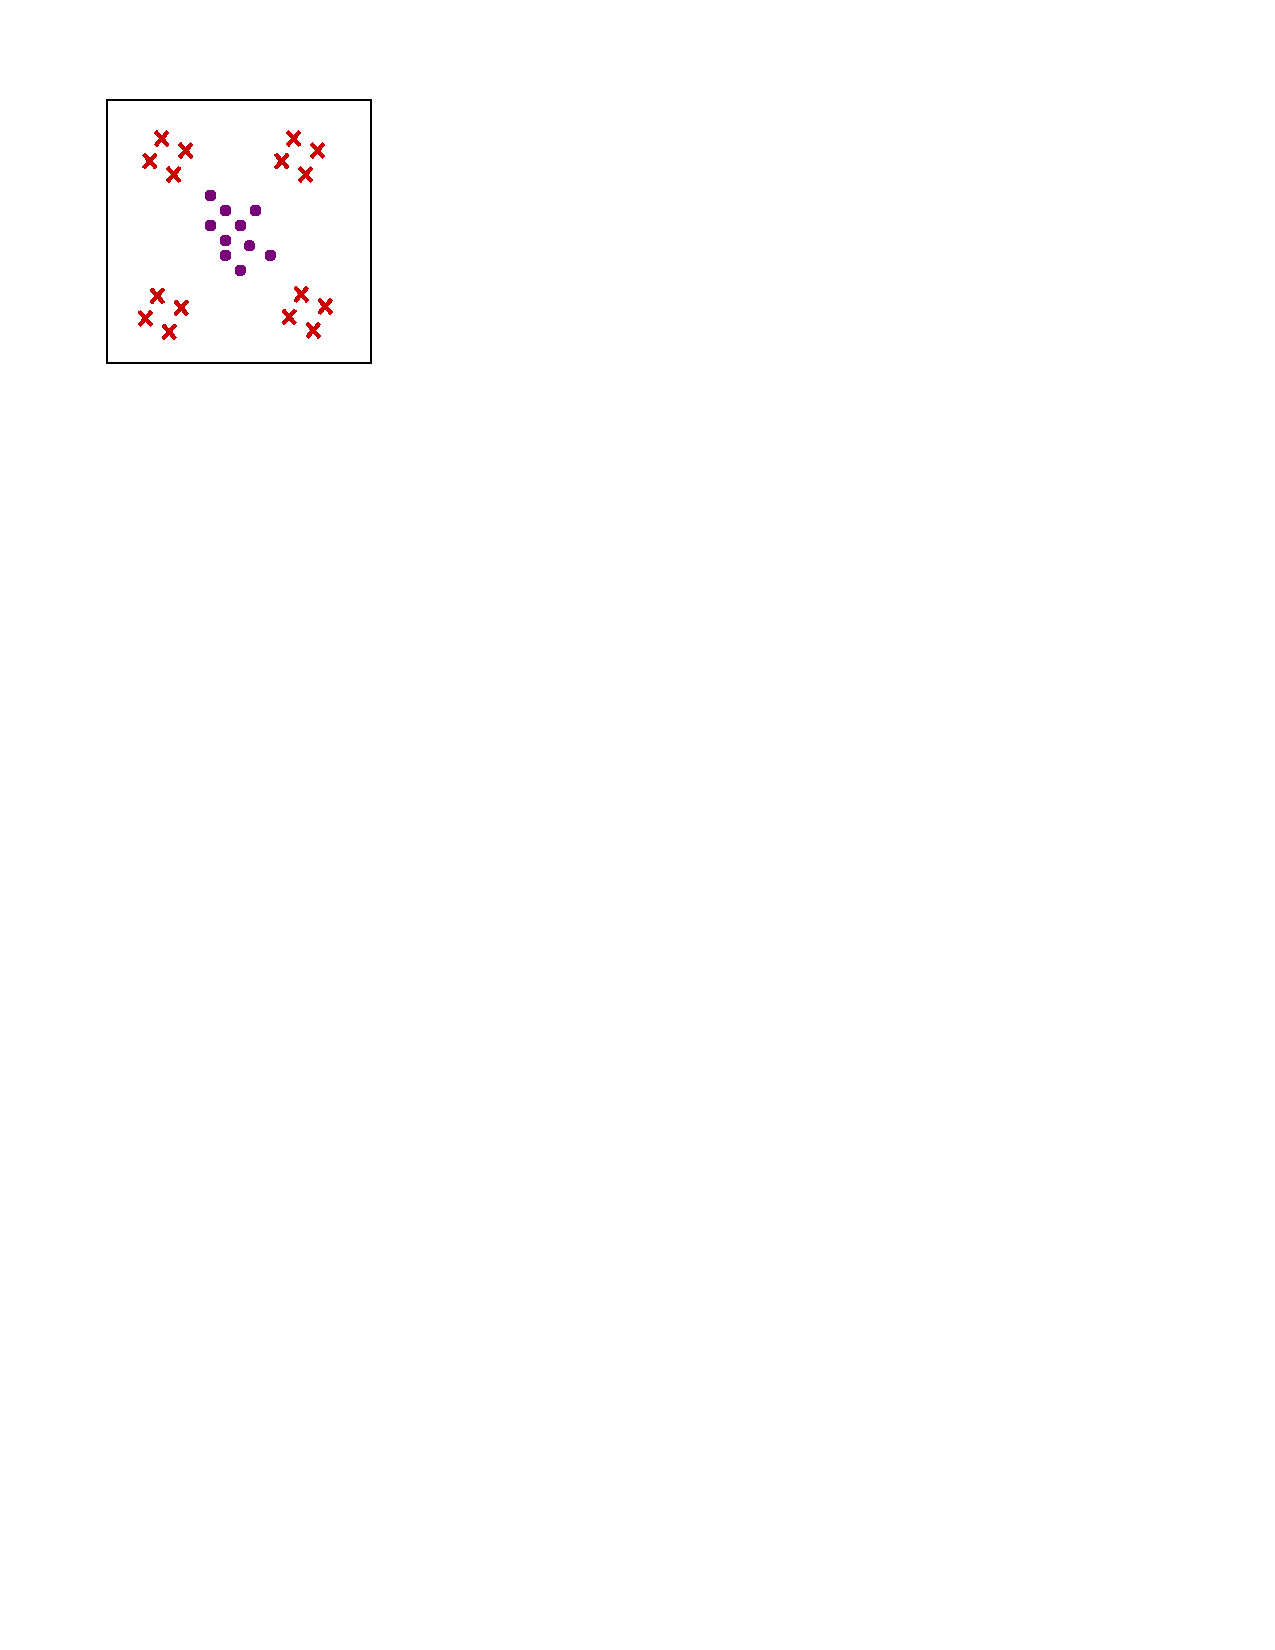
\includegraphics[width=0.35\textwidth]{SVM019}~~~~~~~~~~~~~~~~~~
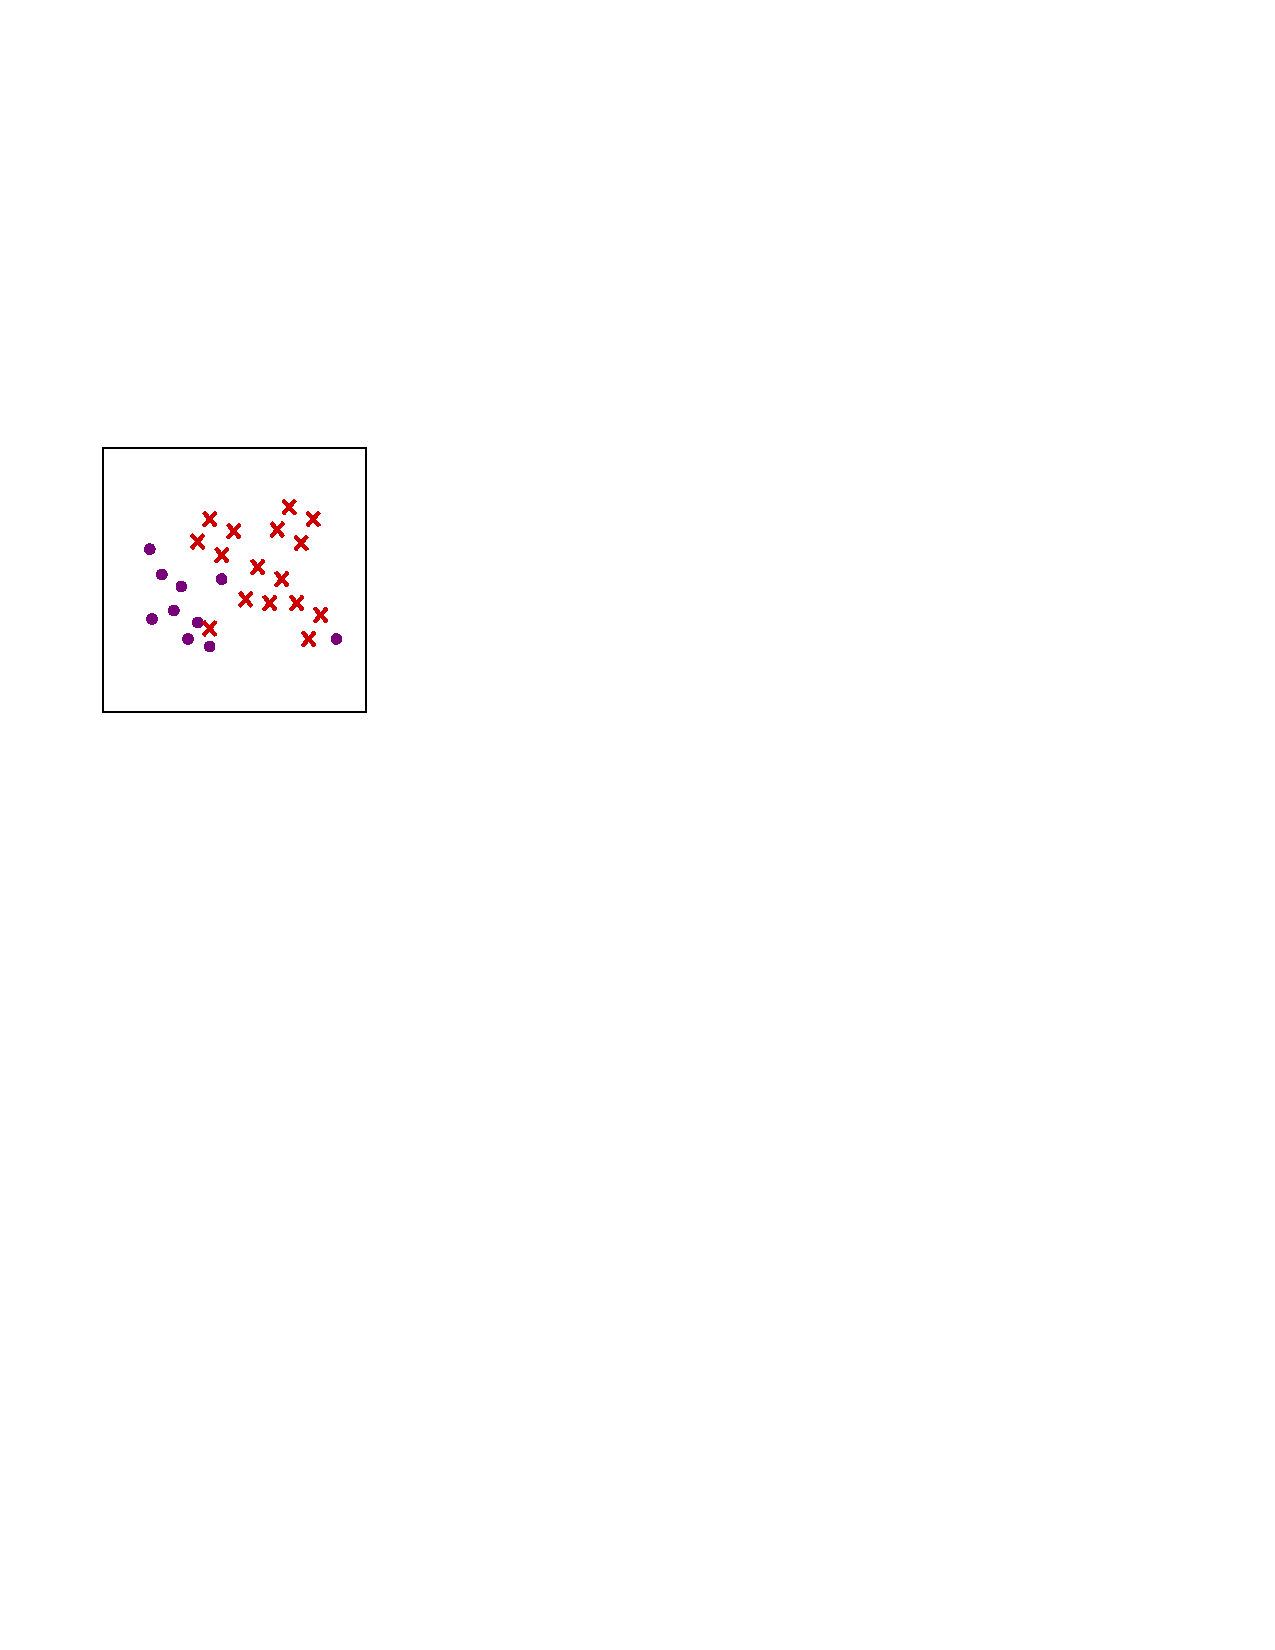
\includegraphics[width=0.35\textwidth]{SVM020}
\end{figure}
\end{frame}

\section{Kernel Trick}
\subsection{}
\begin{frame}{Kernel trick: ${\rm z}$ instead of ${\rm x}$}
\begin{itemize}
\item Dual problem:
\[\boxed{\mathcal{L}(\alpha ) = \sum_{n=1}^{n}\alpha_n -\frac{1}{2}\sum_{i=1}^{n} \sum\limits_{j= 1}^n y_iy_j\alpha_i\alpha_j {\rm z}_i^T{\rm z}_j}\]
Maximize w.r.t. to $\alpha$ subject to $\alpha_i\geq 0$ for $i=1,\ldots,n$ and $\sum_{i=1}^n\alpha_iy_i =0$
\begin{figure}
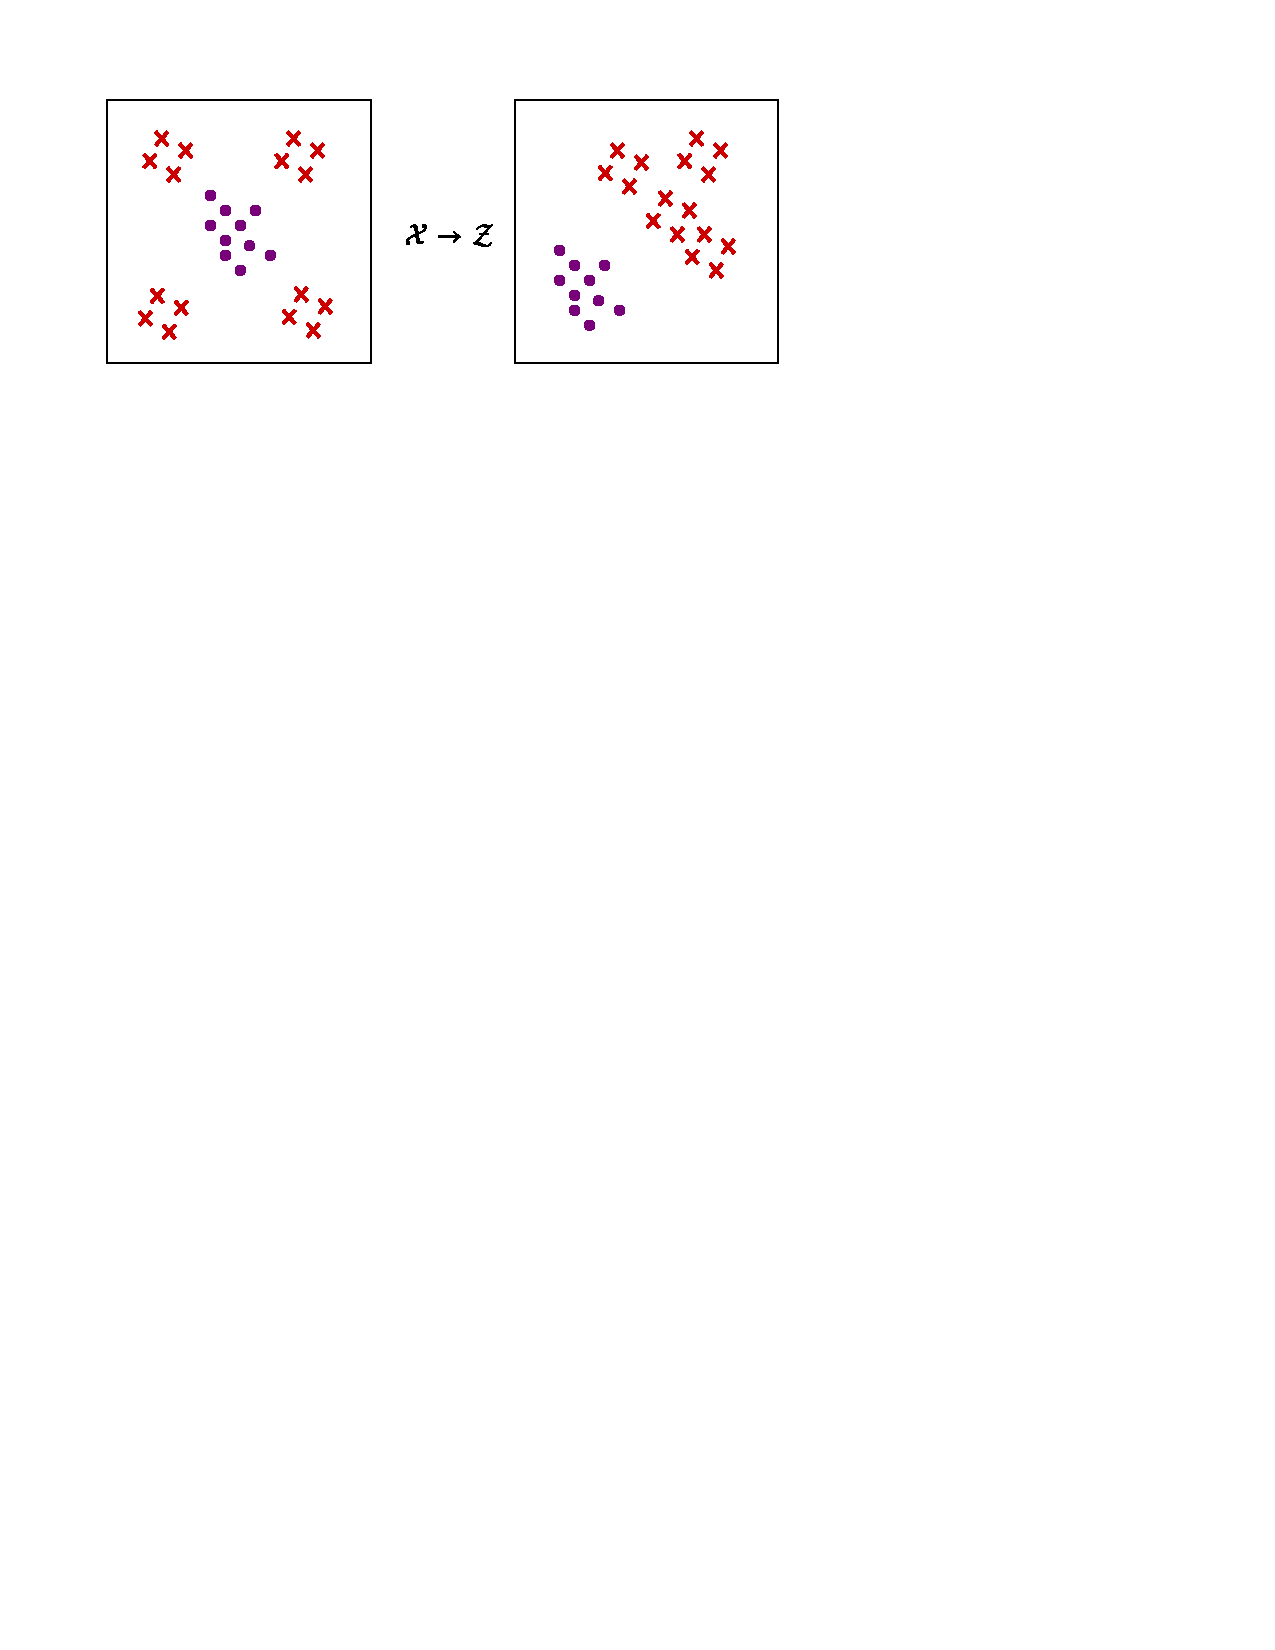
\includegraphics[scale=0.8]{Figures/SVM07.pdf}
\end{figure}
\end{itemize}
\end{frame}

\begin{frame}{Kernel Trick: What do we need from the $\mathcal{Z}$ space?}
\[\boxed{\mathcal{L}(\alpha ) = \sum_{n=1}^{n}\alpha_n -\frac{1}{2}\sum_{i=1}^{n} \sum\limits_{j= 1}^n y_iy_j\alpha_i\alpha_j {\rm z}_i^T{\rm z}_j}\]

Constraints: $\alpha\geq 0\text{~~for~~}i=1,\ldots,n$ and $\sum_{i=1}^{n}\alpha_i y_{i}=0$
\[\boxed{g({\rm x})=\text{sign}({\rm w}^T{\rm z}+b)}~~~~~~ \text{need}~~~~{\rm z}_i^T{\rm z}\]

where
 \[{\rm w}=\sum\limits_{{\rm z}_i\text{ is SV}} \alpha_i y_{i}z_{i}\]

and $b$:
\[y_{j}({\rm w}^T{\rm z}_j+b)=1~~~~~~\text{need  }  {\rm z}_i^T{\rm z}_j\] 
\end{frame}

\begin{frame}{Kernel Trick: generalized inner product}
\begin{itemize}
\item Given two points ${\rm x}$ and ${\rm x}'\in \mathcal{X}$, we need ${\rm z}^T{\rm z}'$.
\item Let ${\rm z}^T{\rm z}'=K({\rm x},{\rm x}')$   (the kernel: inner product of ${\rm x}$ and ${\rm x}'$)
\item Example: ${\rm x}=(x_1,x_2)^T\rightarrow $ 2nd-order $\Phi$
\[{\rm z}=\Phi({\rm x})=(1,x_1,x_2,x_1^2,x_2^2,x_1x_2)\]
\[K({\rm x},{\rm x}')={\rm z}^T{\rm z}'=1+x_1x_1'+x_2x_2'+x_1^2{x'}_1^2+x_2^2{x'}_2^2+x_1{x'}_1x_2{x'}_2\]
\end{itemize}
\end{frame}

\begin{frame}{Kernel Trick}
\begin{itemize}
\item Can we compute $K({\rm x},{\rm x}')$ without transforming ${\rm x}$ and ${\rm x}'$?
\item Consider: 
\begin{align*}
K({\rm x},{\rm x}') &= {(1 + {{\rm x}^T}{\rm x}')^2} = {(1 + {x_1}x'{_1} + {x_2}x'{_2})^2}\\
&= 1 + x_1^2x'{_1}^2 + x_2^2x'{_2}^2 + 2{x_1}x'{_1} + 2{x_2}x'{_2} + 2{x_1}x'{_1}{x_2}x'{_2}
\end{align*}
\item This is the inner production of
\[(1,x_1^2,x_2^2,\sqrt{2}x_1,\sqrt{2}x_2,\sqrt{2}x_1x_2)\]
\[(1,x'{_1}^2,x'{_2}^2,\sqrt{2}x'{_1},\sqrt{2}x'{_2},\sqrt{2}x'{_1}x'{_2})\]
\end{itemize}
\end{frame}

\begin{frame}{Non-linear Kernels}
\begin{itemize}
\item Following are some basic non-linear kernels:
\begin{itemize}
\item Linear: 
\[{K({{{\rm x}}_i},{{{\rm x}}_j}) = {\rm x}_i^{T}{{\rm x}_j}}\]
\item Polynomial: 
\[K({{\rm x}_i},{{\rm x}_j}) = {({\gamma} {\rm x}_i^{T}{{\rm x}_j} + r)^{d}},{\gamma}  > 0\]
\item Radial basis function: 
\[K({{\rm x}_i},{{\rm x}_j}) = \exp \left( { - {\gamma} {{\left\| {{{\rm x}_i} - {{\rm x}_j}} \right\|}^2}} \right),{\gamma}  > 0\]
\item Sigmoid: 
\[K({{\rm x}_i},{{\rm x}_j}) = \tanh \left( {{\gamma} {\rm x}_i^{T}{{\rm x}_j} + r} \right),{\gamma}  > 0\]
\end{itemize}
where, $\gamma$, $r$, and $d$  are kernel parameters. 
\item These kernels were used in various application
where radial basis function (RBF) kernel is widely adopted as a non-linear kernel due to its capability of mapping the feature vectors from input feature space to infinite dimensional space to handle highly non-linear feature distribution.
\end{itemize}
\end{frame}

\begin{frame}{Kernel formulation of SVM}
\begin{itemize}
\item Remember quadratic programming?
\item The only difference  in quadratic coefficients as:
\end{itemize}
\[\begin{gathered}
  \mathop {\min }\limits_{\color{blue}\alpha}  ~~~ \frac{1}{2}{{\color{blue}\alpha}  ^T}\left[ {\begin{array}{*{20}{c}}
  {{y_1}{y_1}z_1^T{z_1}}&{{y_1}{y_2}z_1^T{z_2}}&{\cdots}&{{y_1}{y_n}z_1^T{z_n}} \\ 
  {{y_2}{y_1}z_2^T{z_1}}&{{y_2}{y_2}z_2^T{z_2}}&{\cdots}&{{y_2}{y_n}z_2^T{z_n}} \\ 
  {\vdots}&{\vdots}&{\ddots}&{\vdots} \\ 
  {{y_n}{y_1}z_n^T{z_1}}&{{y_n}{y_2}z_n^T{z_2}}&{\cdots}&{{y_n}{y_n}z_n^T{z_n}} 
\end{array}} \right]{\color{blue}\alpha}  + \left( { - {1^T}} \right){\color{blue}\alpha}  \hfill \\\\
  \text{subject to   }{{\rm y}^T}{\color{blue}\alpha}   = 0\text{   and   }0 \leqslant {\color{blue}\alpha}   \leqslant \infty  \hfill \\ 
\end{gathered} \]
\end{frame}


\begin{frame}{The final hypothesis}
\begin{itemize}
\item Express $g({\rm x})=\text{sign}({\rm w}^T{\rm z}+b)$ in terms of $K(\_,\_)$
\[{\rm w} = \sum\limits_{{z_n}\text{ in SV}} {{\alpha _n}{y_n}{{\rm z}_n} ~~~~\Rightarrow~~~~ g({\rm x}) = \text{sign}\left( {\sum\limits_{{\alpha _n} > 0} {{\alpha _n}{y_n}K({{\rm x}_n},{\rm x})}  + b} \right)} \]
where 
\[b = {y_j} - \sum\limits_{{\alpha _i} > 0} {{\alpha _i}{y_i}K({x_i},{x_j})} \]
for any support vector ($\alpha_i>0$)
\end{itemize}
\end{frame}


\begin{frame}{Problem to be solved: Linear (trivial problem)}
\begin{columns}
\begin{column}{7cm}
\begin{itemize}
\item Suppose we are given the following positively labeled data points in $\Re^2$:
\[\left\{ {\left( {\begin{array}{*{20}{c}}
  3 \\ 
  1 
\end{array}} \right),\left( {\begin{array}{*{20}{c}}
  3 \\ 
  { - 1} 
\end{array}} \right),\left( {\begin{array}{*{20}{c}}
  6 \\ 
  1 
\end{array}} \right),\left( {\begin{array}{*{20}{c}}
  6 \\ 
  { - 1} 
\end{array}} \right)} \right\}\]
\item and the following negatively labeled data points in $\Re^2$
\[\left\{ {\left( {\begin{array}{*{20}{c}}
  1 \\ 
  0 
\end{array}} \right),\left( {\begin{array}{*{20}{c}}
  0 \\ 
  { 1} 
\end{array}} \right),\left( {\begin{array}{*{20}{c}}
  0 \\ 
  -1 
\end{array}} \right),\left( {\begin{array}{*{20}{c}}
  -1 \\ 
  { 0} 
\end{array}} \right)} \right\}\]
\end{itemize}
\end{column}
\begin{column}{7cm}
\begin{figure}
\includegraphics[scale=0.45]{data6.pdf}
\end{figure}
\end{column}
\end{columns}
\end{frame}

\begin{frame}{Solution}
\begin{columns}
\begin{column}{7cm}
\begin{itemize}
\item Since the data is linear separable, we can use a linear SVM.
\item By inspection, it should be obvious that there are three support vectors.
\end{itemize}
\end{column}
\begin{column}{7cm}
\begin{figure}
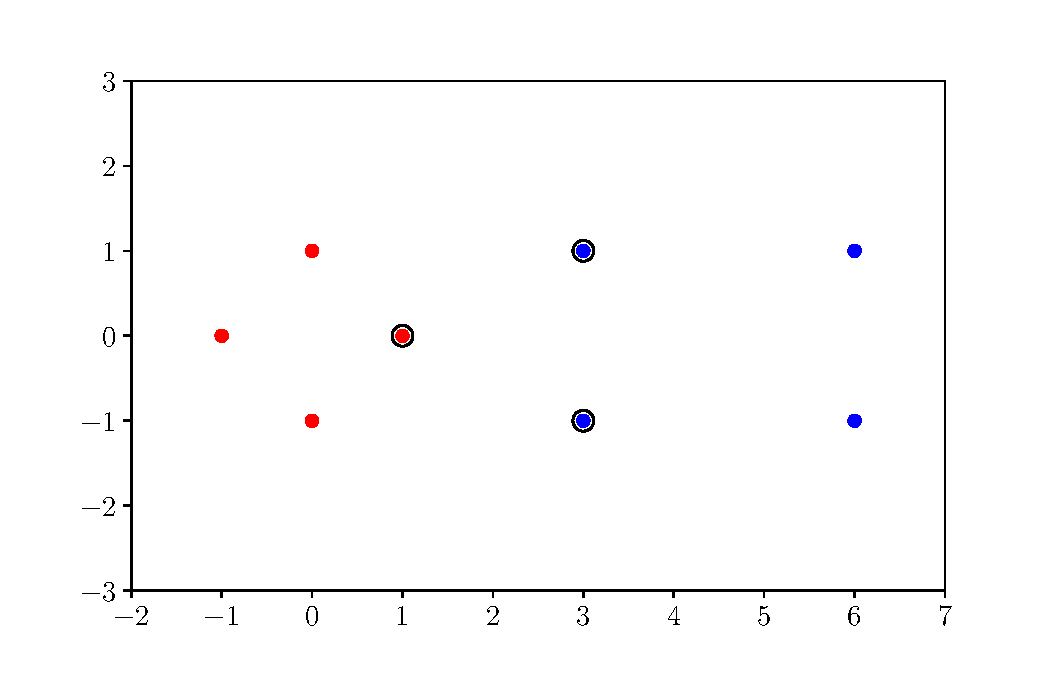
\includegraphics[scale=0.45]{data7.pdf}
\end{figure}
\end{column}
\end{columns}
\end{frame}

\section{Soft Margin Classification}
\subsection{}
\begin{frame}{}
\begin{variableblock}{\centering \Large \textbf{\vspace{4pt}\newline SVM: Soft Margin Formulation\vspace{4pt}}}{bg=slidecolor,fg=white}{bg=slidecolor,fg=white}
\end{variableblock}
\end{frame}

\begin{frame}{Soft Margin Classification}
\begin{columns}
\begin{column}{7cm}
\begin{itemize}
\item In basic SVM, the optimization problem is formulated for margin maximization when the feature vectors are linearly separable. 
\item However, a greater margin can be achieved by {\color{mycolor2}allowing classifier for some misclassification error} during training itself.
\item After allowing the misclassification of some features, the inequality constraint in basic SVM is replaced with ${y_i}({ {\rm w}^T}{\rm x}_i + b) \ge 1-\xi _i$, where $\xi _i\geq 0$ are {\color{mycolor2}slack variables}.
\end{itemize}
\end{column}
\begin{column}{7cm}
\begin{figure}[htbp]
\centering
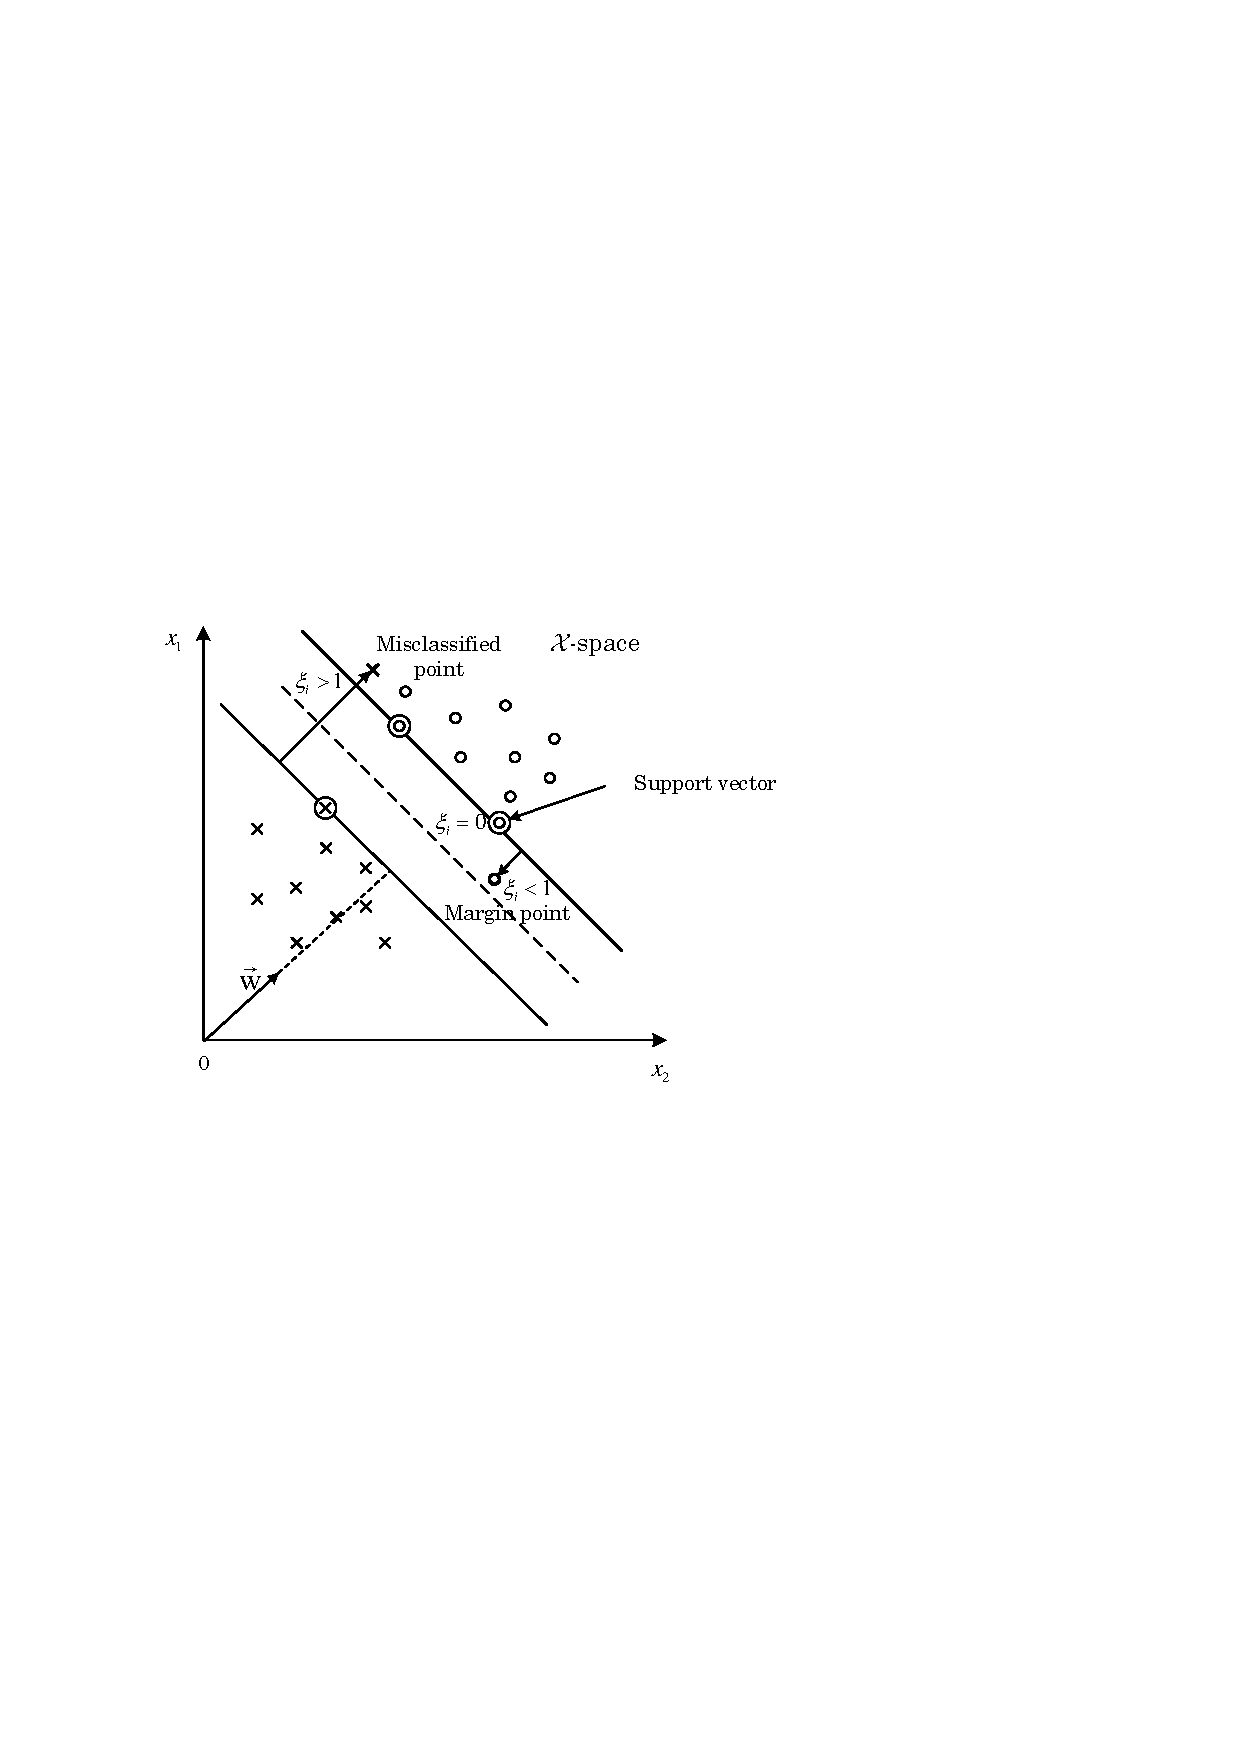
\includegraphics[width=1\textwidth]{SVM}
\caption{$\mathcal{X}$-space with support vector, penalized misclassification, and margin error}
\end{figure}
\end{column}
\end{columns}
\end{frame}

\begin{frame}{The new optimization problem: C-SVM}
\begin{itemize}
\item Slack variables $\xi_i$ can be added to allow misclassification of difficult or noisy examples, resulting margin called soft.
\item Slack variables account for the misclassification and margin errors.
\item The primal optimization problem with
penalized misclassification and margin error becomes.
\begin{equation}
\begin{array}{l}
\mathop {\rm minimize}\limits_{{{\rm w}},b} ~~~~~~\frac{1}{2}{\left\| {{\rm w}} \right\|^2} + C\sum\limits_{i = 1}^{n} {{\xi_i}} \\
{\rm subject~to}:~~~{y_i}({\rm w^{T}}{\rm x}_i + b) \ge 1 - {\xi_i},~{\rm and} \\ ~~~~~~~~~~~~~~~~~~~{\xi_i} \ge 0,~i = 1,2,\ldots,{n},
\end{array}
\end{equation}
\item where C is a regularization parameter which sets the trade-off between margin maximization and minimizing the amount of slack (misclassifications and margin error). 
\end{itemize}
\end{frame}


\begin{frame}{Lagrange formulation}
Using Lagrange multipliers, the dual problem is expressed in terms of Lagrangian coefficients as
\[\mathcal{L}({\rm w},b,\xi ,\alpha ,\beta ) = \frac{1}{2}{{\rm w}^T}{\rm w} + C\sum\limits_{i = 1}^n {{\xi _i} - \sum\limits_{i = 1}^n {{\alpha _i}({y_i}({{\rm w}^T}{{\rm x}_i} + b) - 1 + {\xi _i}) - \sum\limits_{i = 1}^n {{\beta _i}{\xi _i}} } } \]
Minimize w.r.t. ${\rm w}$, $b$, and $\xi$  and maximize w.r.t. each $\alpha_n\geq 0$ and $\beta_n\geq 0$
\[{\nabla _{\rm w}}L = {\rm w} - \sum\limits_{i = 1}^n {{\alpha _i}{y_i}{{\rm x}_i} = 0} \]
\[\frac{{\partial L}}{{\partial b}} =  - \sum\limits_{i = 1}^n {{\alpha _i}{y_i} = 0} \]
\[\frac{{\partial L}}{{\partial {\xi _i}}} = C - {\alpha _i} - {\beta _i} = 0\]
\end{frame}

\begin{frame}{and the solution is ...}
\[\text{Maximize}~~~ \mathcal{L}(\alpha ) = \sum\limits_{i = 1}^n {{\alpha _i} - \frac{1}{2}\sum\limits_{i = 1}^n {\sum\limits_{j = 1}^n {{y_i}{y_j}{\alpha _i}{\alpha _j}{\rm x}_i^T{{\rm x}_j}\text{           w.r.t. to }\alpha } } } \]
\[\text{subject to }0 \leqslant {\alpha _i} \leqslant C\text{ for }n = 1, \ldots ,N\text{               and                }\sum\limits_{i = 1}^n {{\alpha _i}{y_i} = 0} \]
\[ \Rightarrow ~~{\rm w} = \sum\limits_{i = 1}^n {{\alpha _i}{y_i}{{\rm x}_i}} \]
\[\text{minimize}~~~~~~~\frac{1}{2}{{\rm w}^T}{\rm w} + C\sum\limits_{i = 1}^n {{\xi _i}} \]
\end{frame}

\begin{frame}{}

\end{frame}

%\begin{frame}{Types of support vectors}
%\begin{figure}
%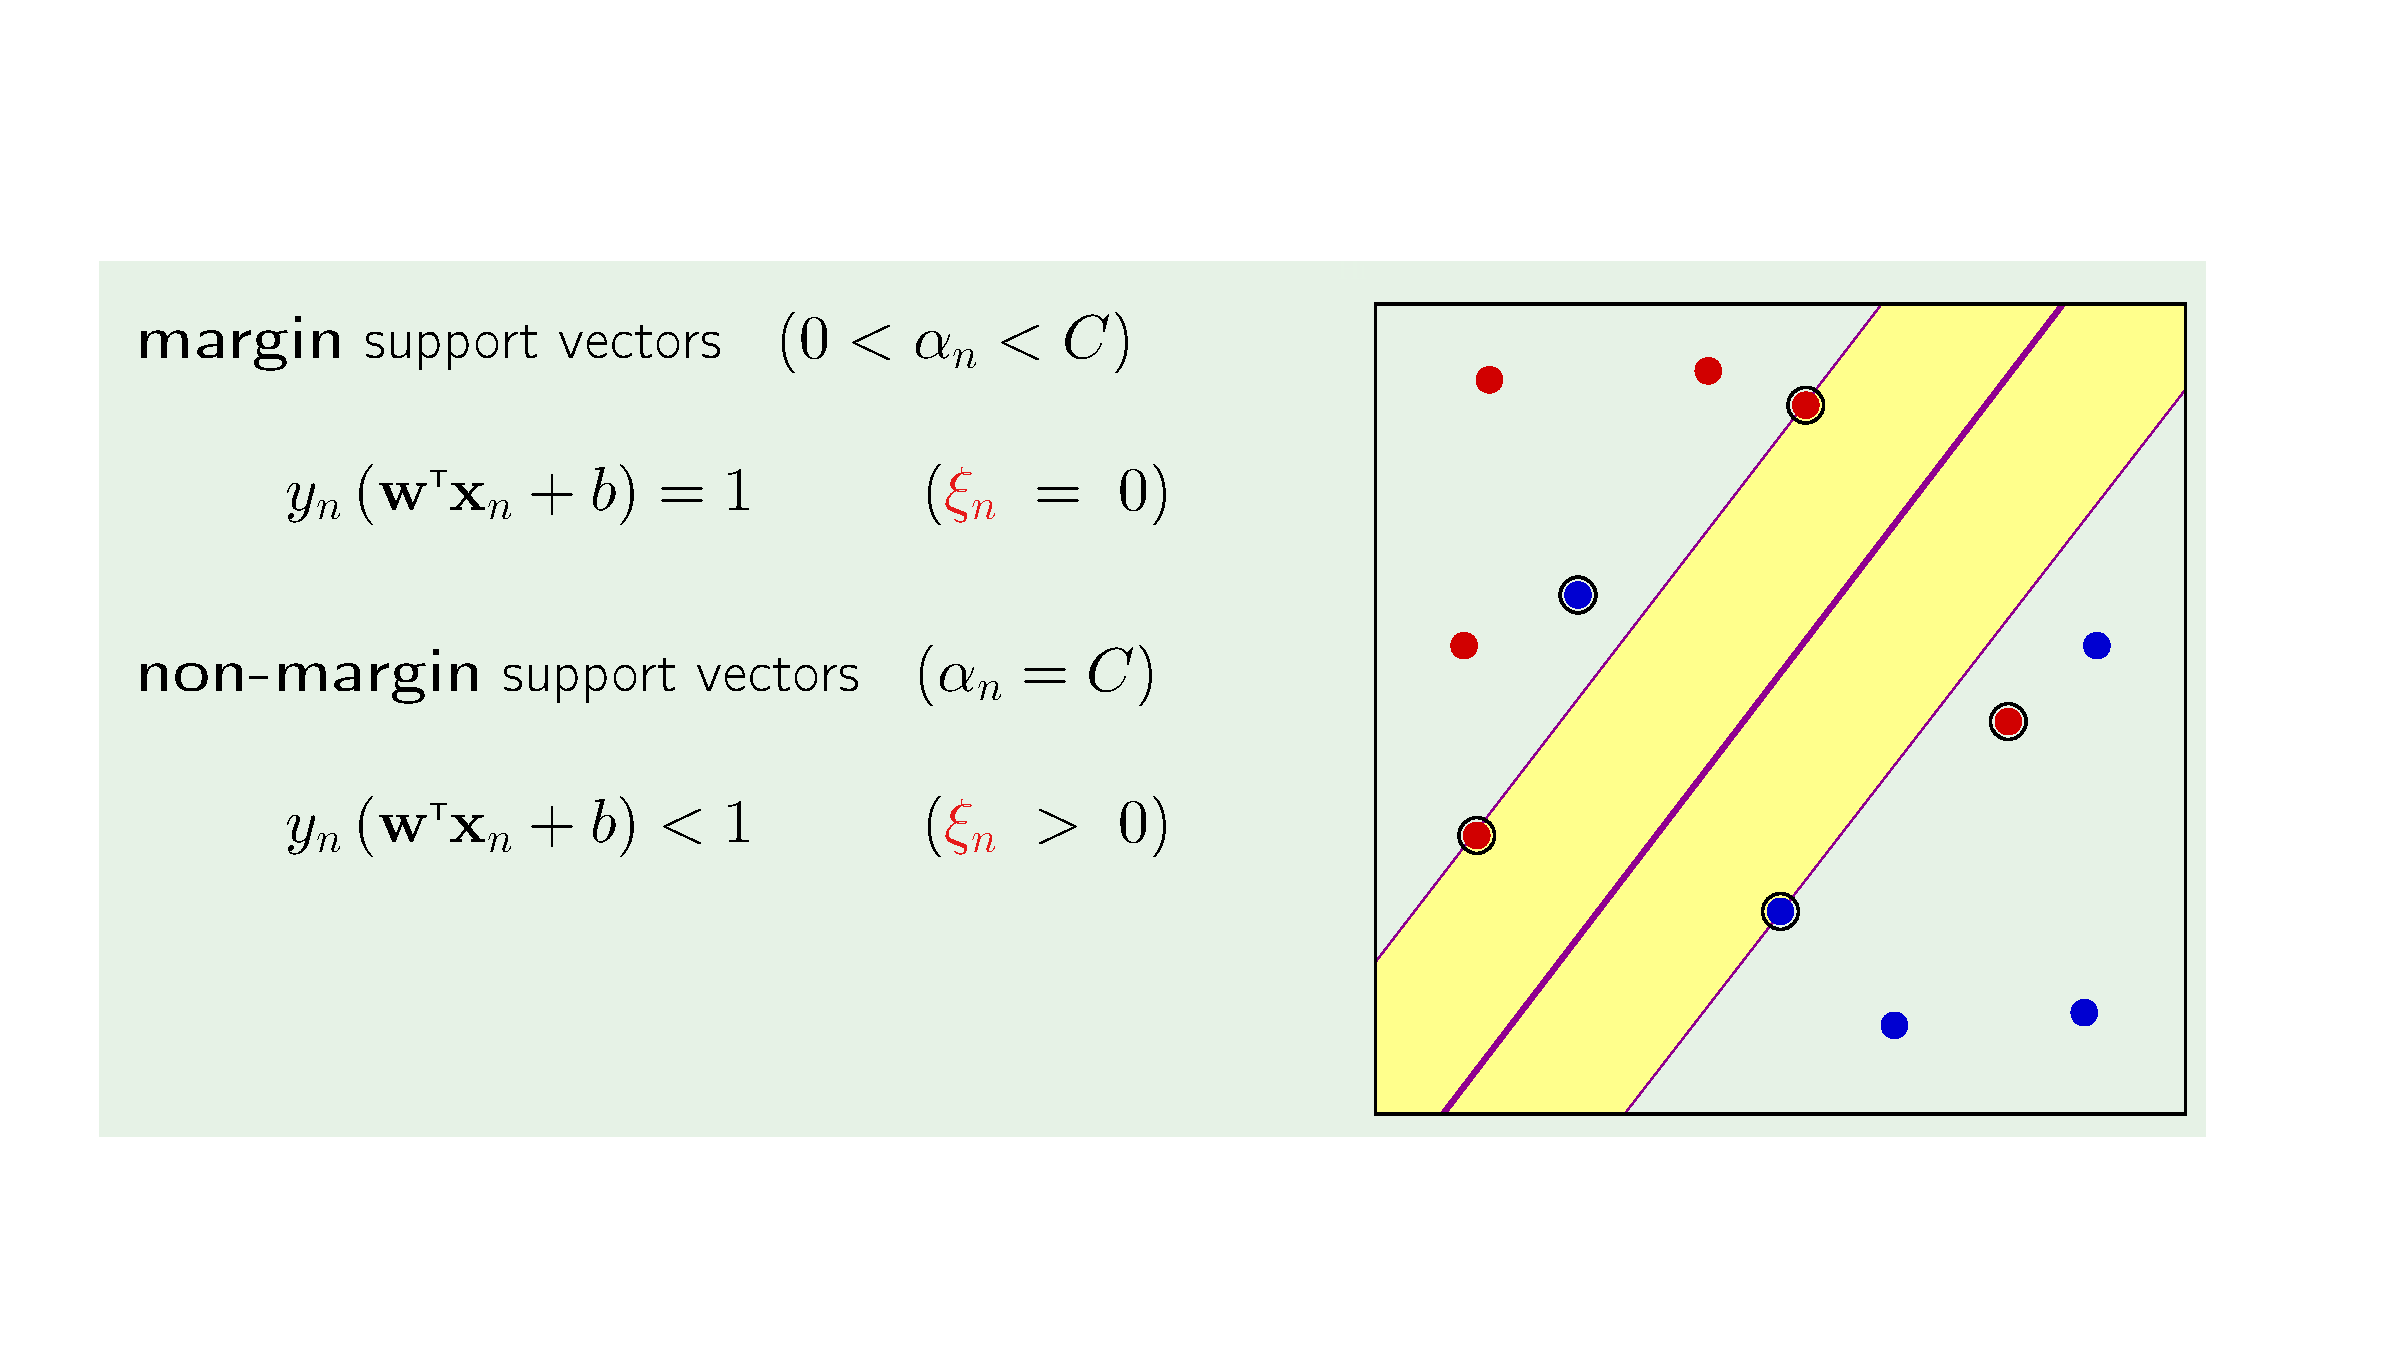
\includegraphics[width=\textwidth]{SVM27}
%\end{figure}
%\end{frame}
%
%\begin{frame}{Two technical observations}
%\begin{figure}
%\includegraphics[width=\textwidth]{SVM28}
%\end{figure}
%\end{frame}

\section{References}
\subsection{}
\begin{frame}[allowframebreaks]{References}
\linespread{1}
\footnotesize
\printbibliography[heading=none]
\end{frame}
{
\setbeamertemplate{logo}{}
\makeatletter
\setbeamertemplate{footline}{
        \leavevmode%
  
  % First line.
  \hbox{%
  \begin{beamercolorbox}[wd=.2\paperwidth,ht=\beamer@decolines@lineup,dp=0pt]{}%
  \end{beamercolorbox}%
  \begin{beamercolorbox}[wd=.8\paperwidth,ht=\beamer@decolines@lineup,dp=0pt]{lineup}%
  \end{beamercolorbox}%
  } %
  % Second line.
  \hbox{%
  \begin{beamercolorbox}[wd=\paperwidth,ht=\beamer@decolines@linemid,dp=0pt]{linemid}%
  \end{beamercolorbox}%
  } %
  % Third line.
  \hbox{%
  \begin{beamercolorbox}[wd=.1\paperwidth,ht=\beamer@decolines@linebottom,dp=0pt]{}%
  \end{beamercolorbox}%
  \begin{beamercolorbox}[wd=.9\paperwidth,ht=\beamer@decolines@linebottom,dp=0pt]{linebottom}%
  \end{beamercolorbox}%
  }%
        }
\makeatother

\begin{frame}
\centering
\includegraphics[width=0.34\paperwidth]{queries.jpg}\\
\includegraphics[width=0.45\paperwidth]{thank_you.png}
\end{frame}
}
